\documentclass[a4paper,11pt,oneside]{report}
\usepackage[T1]{fontenc}
\usepackage[utf8]{inputenc}
\usepackage[francais]{babel}
\usepackage{graphics}
\usepackage{sidecap}
\usepackage{float}
\usepackage[toc,page]{appendix}
%\floatstyle{boxed}
%\restylefloat{figure}
\usepackage{euscript}
\usepackage{url}
\usepackage{amsmath}
\usepackage{amssymb}
\usepackage{amsfonts}
\usepackage{graphicx}
\usepackage{verbatim}
\usepackage{listings}
\usepackage{array}
\usepackage{minted}
\usepackage{placeins}
\usepackage{enumitem}
\usepackage[hidelinks]{hyperref}
\usepackage{colortbl}
\usepackage{multirow}
%\usepackage{moreverb}
\usepackage{tikz}

\usepackage{a4wide}
%\documentclass{article}
%\usepackage[demo]{graphicx}
\usepackage{caption}
\usepackage{subcaption}

\author{Badr ELOUIZ}
\title{Rapport de Stage PFE chez FY Computing}

\begin{document}
\sloppy

\makeatletter
  \begin{titlepage}
  \centering
  
    \begin{figure}[t]
        \begin{tabular}{c c c}
            \multirow{7}{*}{
\includegraphics[scale=0.45]{HASS.png}} & &             \multirow{7}{*}{
\includegraphics[scale=0.35]{logens.png}}\\
             & & \\
             & \textsc{Université Hassan Premier} & \\
             & \textsc{\'Ecole Nationale des Sciences Appliqu\'ees} & \\
             & \textsc{de Khouribga} & \\
             & & \\
             & & \\
        \end{tabular}
    \end{figure}
        \vfill
    {\LARGE \textbf{M\'EMOIRE DE PROJET DE FIN D'\'ETUDES}}\\
        \vspace{0.5em}
    {\large \textbf{Pour l'obtention du}}\\
        \vspace{0.5em}
    {\LARGE \textbf{Diplôme d'Ingénieur d'\'Etat}}\\
        \vspace{0.5em}
    {\large \textbf{Spécialité}}\\
        \vspace{0.5em}
    {\LARGE \textbf{G\'enie Informatique}}\\
        \vfill
    {\large \textbf{Sujet :}}\\
        \vspace{1em} 
    \begin{tabular}{|c|}
    \hline
     \\
    \ \ \ {\LARGE \textbf{Automatisation du Processus de Développement}}\ \ \ \\
    {\LARGE \textbf{des Applications / DevOps}}\\
     \\
    \hline
    \end{tabular}
    \vfill
         {\large \textbf{Réalisé par :}}\\
        \vspace{0.5em}
    {\large \@author} \\
        \vfill
    \begin{tabular}{c c}
    \multicolumn{2}{c}{{\large \textbf{Encadré par :}}} \\
     & \\
    \ \ \ \ {\large M. Youssef BENKIRAN}\ \ \ \ \ \ \ \ \ & \ \ \ \ \ {\large M. Said EL KAFHALI} \\
    \ \ \ \ {\large Ingénieur Informatique,}\ \ \ \ \ \ \ \ \ & \ \ \ \ \ {\large Professeur à l'ENSA de Khouribga,}\\
    \ \ \ \ {\large FY Computing.}\ \ \ \ \ \ \ \ \ & \ \ \ \ \ {\large Université Hassan I de Settat.}\\
    \end{tabular}
        \vfill
    {\large \textbf{Soutenu le 10 Juillet 2017 devant le jury composé de :}}\\
    \ \newline
        $\begin{array}{l l l}
        \text{M. Imad HAFIDI} & \text{Professeur à l'ENSA de Khouribga} & \text{(Président)} \\
        \text{M. Omar EL BENNAY} & \text{Professeur à l'INSA de Khouribga} & \text{(\'Examinateur)} \\
        \text{M. Said EL KAFHALI} & \text{Professeur à l'ENSA de Khouribga} & \text{(\'Encadrant)} \\
        \end{array}$\\
        \vfill
    {\large \textbf{Année universitaire : 2016/2017}}
  \end{titlepage}

\makeatother

\newpage

\ \newline

\newpage

\chapter*{Dédicaces}

\newpage

\chapter*{Remerciements}

\newpage

\chapter*{Résumé}

\newpage

\chapter*{Abstract}

\newpage

\tableofcontents

\newpage

\listoffigures

\newpage

\chapter*{Liste des Tableaux}

\newpage

\chapter*{Introduction Générale}

\newpage

\chapter{Présentation de l'Organisme d'Accueil}

\newpage

FY COMPUTING, est  une entreprise créée en Janvier 2013, basée à Rabat et spécialisée dans l’Informatique de pointe et le Smart COMPUTING, lancée par Emy Capital, holding d’investissement de  Mr. Yahya EL MIR, ex-président et directeur général du groupe SQLI, et présidée par  Mr. Mohammed Feidi BOUZAGBAH, co-fondateur et directeur général. 
\newline
\newline
La spécialisation de FY COMPUTING dans un tel domaine n’est pas anodine puisque l’arrivée de l’internet a progressivement développé une troisième ère de l’Informatique qui est « l’Informatique pour le grand public ».          
\newline
\newline
La  société propose des nouvelles technologies et des services de haut niveau destinés, aux entreprises et au grand public. Parmi ces solutions on trouve :

\begin{itemize}
\item \textbf{iWay :} Digital Vision from Strategy to Execution Governance \& Mentoring  Monitor.
\item \textbf{iWalk :} Digital IT Smart Project Catalog Services platform Express Rollout.
\item \textbf{iWheel :} C'est un modèle pour piloter la transformation digitale. Il est conçu sur trois principes :

\begin{itemize}
\item Une démarche apprenante qui permet aux entreprises de tester rapidement de nouveaux concepts et d’en tirer les enseignements.

\item Un modèle de maturité digitale basé sur les principes du « Total Quality Management ». Les entreprises peuvent ainsi faire évoluer leur culture digitale et leur organisation de manière structurée et progressive.

\item Les meilleurs outils et pratiques générés par la richesse des écosystèmes afin de gagner du temps et accélérer les capacités digitales.
\end{itemize}
\end{itemize}

\section{Les Valeurs de FYComputing}
Parmi les valeurs de l’entreprise FY COMPUTING on trouve : 

\begin{itemize}
\item \textbf{Le goût de l’innovation :}

L’entreprise cherche en permanence à offrir des produits/services uniques sur le marché et dont les clients ne pourront pas s’en passer.

\item \textbf{La culture du partenariat :}

Pour innover, aller vite, satisfaire ses clients finaux, obtenir des résultats, un écosystème de bons partenaires fiables et pointus dans leur domaines est indispensable. Cela oblige à avoir des partenaires qui naturellement ont le goût de l’excellence et du travail bien fait.

\item \textbf{Santé financière :}

FY COMPUTING considère la santé financière d’une entreprise comme la santé physique d’une personne. Vous ne pouvez réellement entreprendre et aller au bout de vos idées sans une bonne santé. C’est la raison pour laquelle elle est dotée d’un positionnement basé sur l’excellence et d’un business model solide, garantissant la bonne santé financière de l’entreprise et son indépendance.
\end{itemize}


\section{Positionnement de FY COMPUTING}
Le digital transforme la façon de produire, de vendre et de communiquer. La révolution digitale impose de nouveaux usages impactant les entreprises, leur modèle, leur management, l’ensemble de leurs métiers, et cela quel que soit le secteur d’activité. Les règles du jeu changent, l’IT doit s’adapter. Les entreprises ont besoin de partenaire agile capable de les alimenter en innovation et de répondre aux nouveaux usages et attentes de leurs clients. Le positionnement de FY COMPUTING est de répondre à ces nouvelles exigences.
\newline
\newline
Simplifier l’informatique pour les clients dans des domaines stratégiques très complexes telle pourrait être résumée la mission de FY COMPUTING. Ceci définit ses domaines d’activités comme suit :

\subsection{La Transformation Digitale}
L’accélération des mutations technologiques et l’évolution rapide des usages des outils informatiques marquent le marché marocain aujourd'hui, la technologie s’immisce aujourd’hui à travers l’ensemble de ces silos, dans toutes les couches de l’entreprise, jusqu’au cœur de la relation client. En rapprochant les fonctions, quand elle ne permet pas de les fusionner, la technologie est un levier saisissant d’amélioration des processus. Elle ouvre de nouvelles opportunités pour l’organisation. Ainsi la digitalisation des processus de transformation non seulement le business model (le développement de nouveaux produits, nouveaux services numériques ou objets connectés ; Diversification dans les activités numériques), les services et les opérations (Développement de nouveaux canaux d’interaction, Personnalisation de la relation client, Digitalisation des processus et des opérations terrain) , mais également le working model (Digitalisation des processus internes, Adaptation des organisations au travers de nouveaux modèles de travail et des systèmes de management, Développement de compétences numériques).
\newline
\newline
Intelligence stratégique, excellence opérationnelle et connaissance approfondie, sont les clés de la réussite d’une transformation digitale. En revanche, il faut piloter cette transformation avec différents modèles de gouvernance en s’adaptant à la maturité de l’entreprise. C’est une approche coordonnée qui doit être alignée avec une vision et une stratégie. C’est pour cela qu’elle doit se faire avec l’appui de la direction générale et du département informatique, qui va standardiser tous les processus. Cette transformation globale de l’entreprise doit se faire de façon cohérente par rapport aux métiers. Une bonne transformation digitale touche les clients, les services, les fournisseurs, etc. C’est comme une économie intégrée.
\newline
\newline
Inscrites dans cette ère, FY COMPUTING en collaboration avec iRévolution ont lancé iWheel, modèle de maturité digitale permettant aux entreprises de piloter leur transformation digitales.

\subsection{Smart Computing}
Le Smart Computing est une informatique plus simple, plus amusante, plus fiable qui a permis à de petites entreprises de devenir des géants en seulement une décennie. Il peut être défini comme l'état d'un système d'information qui permet de fournir, au moment approprié ou dans un contexte donné, l'ensemble des informations (internes ou externes), leur synthèse et les analyses utiles, afin que son utilisateur prennent les décisions pertinentes, et entreprennent les actions utiles, à la réussite de sa fonction. Il ne s'agit donc pas simplement d'un outil spécifique, mais d'une organisation fonctionnelle de l'emploi de l'outil informatique, qui peut être optimisé par des logiciels non structurants.
\newline
\newline
Par sa nature, le Smart Computing n'est pas techniquement structurant, et n’impacte pas les choix d’architecture de la direction informatique. Il ne l'est pas non-plus de la fonction RH. Sa vocation à libérer l'opérateur des tâches informatiques sans valeur ajoutée, s'exprime dans sa facilité d'utilisation, son absence de besoin en formation, sa caractéristique à s'auto contrôler au service de l'utilisateur.
\newline
\newline
Dès lors il permet un remarquable taux d'acceptabilité des personnels et de leurs organisations représentatives. Derrière l'avancée technique, il est perçu comme une véritable avancée sociale qui valorise le travail utile, conforte la performance et améliore l'implication des personnels. Ce confort dans le travail est apprécié positivement par les syndicats des grandes entreprises qui en ont fait l'expérience.
\newline
\newline
Le Smart Computing est enfin une réponse pertinente aux besoins en RH dans la gouvernance de l'entreprise. Celles-ci sont sous la pression croissante et les exigences pointilleuses des règlementations, des ONG, et des clients. La concurrence accrue et le rythme accéléré des avancées technologiques imposent aux organisations d'augmenter leur capacité à innover et produire avec une agilité maîtrisée.
\newline
\newline
Les prospectives d'investissement des grands comptes placent le Smart Computing comme l'une des 10 technologies porteuses de ces prochaines années. Il conviendrait également de placer cette technologie comme un investissement créateur de valeur dans la ressource humaine, tant ses effets positifs apportent à cette fonction.
\newline
\newline
Etant inscrites dans ce contexte, FY COMPUTING \& iRevolution ont uni leurs compétences pour créer Smart Project, une innovation destinée aux grands groupes qui veulent bénéficier des avantages du Smart Computing. Cette innovation se remarque sur plusieurs points lors de la réalisation d’un projet à savoir :

\subsection{Des Nouvelles Façons Motivantes de Travailler}
S’il est une chose dont l’informatique d’entreprise traditionnelle ne manque pas, ce sont les nombreux documents : cahiers des charges, spécifications, dossiers techniques, grilles et des piles de documentation. Tout cela est de nature à rassurer les ingénieurs et les consultants mais ne crée pas la motivation et la stimulation dont les équipes business ont besoin. Et quand en plus, le résultat n’est pas au rendez-vous, la déception est à la hauteur de l’effort consenti. « L’un des aspects les plus merveilleux de Smart Project, c’est qu’il permet d’obtenir des résultats spectaculaires et très remarquables. Auparavant, le premier critère pour juger une marque était la qualité du produit ; désormais, c’est la qualité de l’expérience qui importe avant tout. » explique Grégory Pallière, D.G d’iRévolution.

\subsection{Bâtir un Pont entre le Business et la Technologie}
« Smart Project révolutionne non seulement notre façon de gérer les projets, mais aussi la façon de travailler de toute l’équipe », explique Mohamed Feidi BOUZAGBAH. « Pour chaque projet, l’une de nos priorités est de bâtir un pont entre la technologie et le business auquel le projet est destiné. Smart Project nous aide à atteindre cet objectif » ajoute-il, « Pour nous, Smart Project n’est pas juste un moyen de faire des économies ni de travailler plus vite », complète Grégory Pallière. « Il nous aide aussi à améliorer les réponses aux enjeux business à chaque étape de notre travail, ce qui sans cahier des charges, sans spécifications laborieuses, ni réunions fastidieuses ! » déclare Yahya EL MIR.

\subsection{Actions Focalisées, Excellence 2.0}
Les actions de FY COMPUTING sont focalisées sur ce qui est le plus important pour les clients. « La simplicité, c’est la sophistication extrême » disait Steve Jobs. Smart Project met un focus tout particulier sur le design et l’expérience utilisateur. « L’expérience utilisateur est la clé aujourd’hui d’un marketing efficace, et l’expression la plus puissante de cela se traduit par un meilleur produit au final.»

\newpage

\chapter{Contexte du Projet et Problématique}

\newpage

\section{Contexte Général du Projet}

Au sein de l’Entreprise, généralement l'équipe de développement des applications est chargée d’exécuter les missions suivantes : Réaliser une étude des besoins fonctionnels pour élaborer un cahier des charges de l’applications à développer, puis concevoir la partie technique du projet pour ensuite la traduire en code source, ce dernier doît être testé avant la phase de déploiement.
\newline

Le code source développé par l’équipe de développement est souvent testé dans plusieurs environnements avant de le mettre en production; en local, puis en environnement de tests, et enfin dans un environnement de pré-production. Si les test dans un environnement donné sont passés avec succès, l'équipe de développement met le code à la disposition de l’équipe de l’exploitation pour l’exploiter dans l’environnement suivant.
\newline

Ce paradigme pose un problème : lorsque les deux équipes travaillent séparément, le développeur peut ne pas être au courant des obstacles opérationnels qui empêchent le programme de fonctionner comme attendu.
\newline

Ce cloisonnement entre les équipes a un impact non négligeable sur le business :
\begin{itemize}
\item Des applications qui ne fonctionnent pas en production malgré les tests.
\item Une durée de déploiement trop importante.
\item Un « Time To Market » trop important.
\item Une impossibilité de livrer rapidement en production un correctif de bug.
\item Des difficultés à gérer l’ensemble des configurations.
\item Des retards de livraisons.
\item Des problèmes de performance des applications.
\item Des difficultés à augmenter rapidement la capacité d’une application.
\newline
\end{itemize}

Alors pour remédier ce problème, on cherche à fusionner le développement et le déploiement au sein d'un exercice plus rationalisé, c’est ainsi que le mot ‘DevOps’ a apparu pour décrire cette fusion.
\newline

Pour réussir un bon DevOps, il faut également des outils technologiques qui interviennent dans les phases de développement des applications informatiques :

\begin{itemize}
\item \textbf {Gestion du développement :} la production du code s’effectue avec des outils propres aux développeurs :
\begin{itemize}
\item un IDE (environnement de développement intégré) comme Eclipse, WebStorm, Android Studio, Visual Studio, …).
\item un framework de développement (AngularJS, Ruby on Rails,  NodeJS, …).
\item un outil de requêtage SQL (SQLDevelopper, Toad, …). 
\end{itemize}

\item \textbf {Gestion du stockage du code :} le code doit être poussé sur dépôt central permettant la mutualisation entre les développeurs d’une même équipe. Des outils comme Git, GitLab, GitHub, Bitbucket, CVS, Subversion ou Mercurial peuvent ainsi être utilisés.


\item \textbf {Gestion de l’intégration continue (CI) :} Le code doit générer automatiquement des builds à l’aide d’un gestionnaire d’intégration continue comme Jenkins\cite{jenkinsEssentials} (fork de Hudson), TeamCity, CruiseControl, ...


\item \textbf {Gestion des tests :} les tests unitaires ont des outils de la famille xUnit comme Junit (monde Java), JSUnit, PyUnit, etc. Les tests métiers disposent d’outils comme Selenium, Behat, etc. D’autres types de tests doivent être effectués comme les tests de sécurité (OWASP, etc.), les tests de performances (JavaMelody, outils d’APM, JMeter, etc.).
\newline

D’autres outils complètent la panoplie et permettent d’augmenter l’automatisation et ainsi d’améliorer la productivité :

\item Les plateformes IaaS (Amazon AWS, Google App Engine, Mirosoft Azure, etc.) qui vont permettre de provisionner en automatiques les machines virtuelles (VMs) nécessaires au fonctionnement de l’application.
\item Les gestionnaires de configuration (Puppet et Chef, Ansible).
\item Les gestionnaires de Conteneurisation (Docker\cite{proDocker}\cite{usingDocker}).
\end{itemize}

\section{Problématique et Objectifs}

\newpage

\chapter{Concepts Suivis et Technologies Utilisées}

\newpage

\section{Concepts Suivis}

\subsection{Culture DevOps}

\subsection{Infrastructure as Code (IaC)}
Cette partie discute le principe d'\texttt{IaC; Infrastructure as Code}\cite[Chapter~4]{thePracticeOfSystemAndNetworkAdministration} (en français ``\texttt{Infrastructure en tant que Code}''), une stratégie d'administration des systèmes dont l'infrastructure est provisionnée et gérée à travers des fichiers de configurations programmés au lieu du travail manuel. Cette méthode nous permet de gérer nos infrastructures en utilisant les même techniques de développement des applications comme les systèmes de contrôle des versions, tests unitaires, l'Intégration Continue et le Déploiement Continue (CI/CD). 
\newline

Avec le principe d'\texttt{IaC}, on effectue les changements aux systèmes en changeant les fichiers de code et de configuration utilisés, et non directement sur ces systèmes. Le code source utilisé pour décrire notre infrastructure représente notre environnement de travail, il décrit les machines, leurs programmes et applications, les connexions réseaux entre elles ... etc. On développe notre infrastructure la façon comment un développeur produit son application.
\newline

\texttt{IaC} n'est pas un systèmes ni un langage de programmation, c'est un principe et un méchanisme à suivre et implémenter à travers les outils disponibles pour cela; Puppet\cite{puppetWiki}, Chef\cite{chefWiki}, Docker (voir section \ref{docker}) ... etc.

\subsubsection{Avantages d'Infratructure as Code}

Par l'adoption de cette stratégie, on bénificie de trois avantages majeures :
\begin{itemize}
  \item\textbf{\emph{Coût réduit}} : Tout simplement parce que le travail manuel est presque éliminé. L'automatisation permet qu'une personne réalise les tâches de plusieurs, ce qui veut dire moins de personnes employées!
  \item\textbf{\emph{Déploiement rapide}} : Les tâches sont exécutés de manière rapide et en parallèle. 
  \item\textbf{\emph{Moins de risque}} : Moins de risque d'erreurs et bugs en suivant les techniques de développement informatique. Aussi, moins de risque de sécurité avec les différents types de tests automatisés.
\end{itemize}

\subsubsection{Principes d'Infratructure as Code}

Les principes d'\texttt{IaC} sont les suivants :
\begin{itemize}
  \item\textbf{\emph{Tous les changements à travers les fichiers source de configuration}} : Ne pas se connecter aux serveurs pour effectuer les changements, il vaut mieux utiliser les fichiers du code et de configuration.
  \item\textbf{\emph{La documentation à travers le code source}} : Les fichiers de documentation et ses illustrations doivent être générés à partir du code et des fichiers de configuration parce qu'ils sont la source fiable d'architecture de l'infrastructure.
  \item\textbf{\emph{Utilisation d'un système de contrôle des versions}} : Tous les fichiers du code et de configuration doivent être contrôlés par un système de contrôle des versions pour garder l'historique des changements.
  \item\textbf{\emph{Implémentation de l'Intégration / Déploiement Continue (CI/CD)}} : Exécutez les tests et le processus d'automatisation après chaque modification pour identifier les erreurs rapidement puis les corriger. 
  \item\textbf{\emph{Un petit changement à la fois}} : Les erreurs sont simples à trouver lorsqu'elles résident dans un petit changement des fichiers. De même, les petits changements sont plus simple à déploier et/ou annuler que les grands changements.
  \item\textbf{\emph{Le service est toujours disponible}} : Il vaut mieux appliquer des techniques pour garder le service offert disponible aux moments des mises à jour (exemples: la haute disponibilité, la tolérance aux pannes ...). Comme ça on peut effectuer des changement plus fréquemment sinon il sera difficile d'applique le principe précédent!
\end{itemize}

\subsection{Continuous Integration (CI)}

\subsection{Continuous Deployment (CD)}

\subsection{Clustering}

\section{Technologies Utilisées}

\subsection{Docker} \label{docker}
Docker est un logiciel open source qui automatise le déploiement d'applications dans des Conteneurs logiciels. Ceci permet d'étendre la flexibilité et la portabilité d’exécution d'une application, que ce soit sur la machine locale, un cloud privé ou public, une machine nue, etc. 
\newline

Docker étend le format de conteneur Linux standard (LXC) avec une API de haut niveau fournissant une solution de virtualisation qui exécute les processus de façon isolée. Docker utilise LXC, cgroups, et le noyau Linux lui-même. Contrairement aux machines virtuelles traditionnelles, un conteneur Docker n'inclut pas de système d'exploitation,  mais s'appuyant sur les fonctionnalités du système d’exploitation fournies par l'infrastructure sous-jacente.

\subsubsection{Conteneurs vs Machines Virtuelles}
En principe, les Conteneurs sont l'encapsulation d'une application avec ses dépendences. En premier temps, ils apparaissent comme une forme légère des VMs (i.e. Machines Virtuelles). Les deux techniques contiennent un système d'exploitation isolé surlequel on peut déployer nos applications. Cependant, les Conteneurs apportent de nombreux avantages difficiles (voir impossible!) d'avoir avec les VMs :
\begin{itemize}
\item Les Conteneurs partagent les ressources avec le système hôte beaucoup plus efficace que les VMs. 
\item Les Conteneurs peuvent être lancer et arrêter dans des millisecondes. 
La portabilité des Conteneurs élimine le guerre des dépendances inter-systèmes, garantie que ça va marcher indépendamment du système hôte. 
\item Les Conteneurs sont incroyabelement légers permettant aux utilisateurs d'exécuter des dizaines (même plus) de Conteneurs en même temps pour simuler un vrai environnement de production distribué, ce qui n'est pas le cas souvent avec les VMs. 
\item Les clients finaux des applications peuvent télécharger puis exécuter ses applications complexes rapidement sans devoir passer des heures de souffrance des installations et de configurations. 
\newline
\end{itemize}

De plus, l'objectif essentiel d'un Conteneur est de rendre une application complètement portable et autonome, au contraire des VMs qui visent la virtualisation totale d'un environnement externe.

\begin{figure}[H]
    \centering
    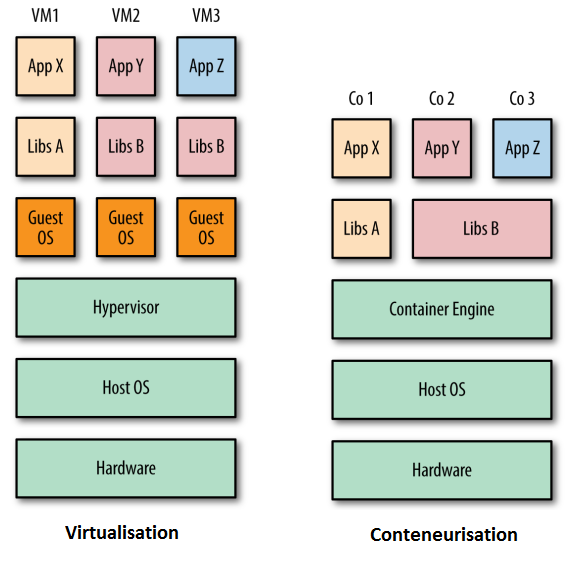
\includegraphics[width=12cm]{vm-vs-container.png}
    \caption{Exemple de trois applications X, Y et Z déployées à gauche à l'aide des VMs et à droite en utilisant des Conteneurs.}
    \label{fig:vm-vs-container}
\end{figure}

\subsubsection{Introduction à Docker}

En réalité, la Conteneurisation existe depuis longtemps sur les systèmes UNIX/Linux sous plusieurs formes ; chroot, jail. Après la création de la technologies open source de conteneurisation OpenVZ (anciennement Virtuozzo) par Parallels Inc. et LXC (Linux Containers) par Google .. et autres, Docker a apporté la pièce manquante de la solution mature et complète en 2013.
\renewcommand{\appendixtocname}{Annexes}

Docker fournit un ensemble de produits et services à savoir :
\begin{itemize}
\item \textbf{Docker Engine} est le moteur de Conteneurisation qui fournit une interface d'execution des Conteneurs simple et efficace. 
\item \textbf{Docker Hub} est un espace Cloud public qui contient des centaines des images Docker créées par la communaté pour partager et commencer rapidement à partir de ce qu'existe déjà. 
\item \textbf{Docker Store} est similaire à Docker Hub mais fournit des Images certifiées  pour les Entreprises (parfois payantes). 
\item \textbf{Docker Swarm}, un gestionnaire des clusters de Conteneurs. 
\end{itemize}

Après l'adoption rapide de la technologie des Conteneurs à l'aide de Docker, ce dernier a devenu le standard dans l'industrie, ce qui a mené à créer l'ogranisation Open Container Initiative par Docker, Google, Microsoft, CoreOS et autres pour normaliser le standard.
\newline

\subsubsection{Principes Docker}

\begin{figure}[H]
    \centering
    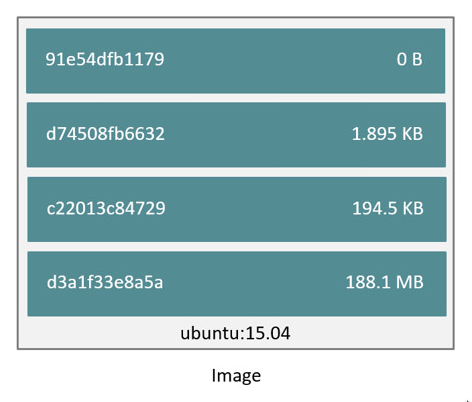
\includegraphics[width=10cm]{ubuntu-image.png}
    \caption{Les couches de système de fichiers d'une Image Docker Ubuntu.}
    \label{fig:ubuntu-image}
\end{figure}

Le fonctionnement Docker se base sur les principe des `Images Docker`. Une Image Docker est la base des Conteneurs Docker. Une Image Docker est une collection ordonnée des changements effectués sur un système de fichiers et de ses paramètres d’exécutions, pour l’utilisation dans un Conteneur en cours d’exécution. Généralement, une Image est l’union des couches – en lecture seule - des systèmes de fichiers stockées l’une au-dessus de l’autre pour former le système de fichiers racine d’un Conteneur. Chacune de des couches est identifiée par un code de hashage unique généré par Docker au moment de construction de l’Image. Les Images Docker n’ont aucun état et ne changent jamais.
\newline

Une Image est construite automatiquement par Docker à partir d’un fichier texte appelé Dockerfile, qui contient un ensemble d’instructions et commandes,  ordonnées, pour construire une telle Image. Dockerfile a un format specifique et accèpte un ensemble d’instructions spécifiques qui définissent le contenu des couches de systèmes de fichiers de l’Image finale. Une Image bien construite est celle qui est légère au maximum possible en contenant seulement les applications nécessaires au fonctionnement du service fournit et le stricte minimum des couches de systèmes de fichiers.
\newline

Pour éviter la répétition, Docker fournit un espace de stockage dans le Cloud gratuit pour partager les Images Docker avec Docker Hub. Récemment, Docker a annoncé son service Cloud payant Docker Store riche en fonctionnalités avancées et destiné aux Entreprises. Ceci permet de démarrer rapidement avec Docker en exploitant des centaines d’Images publiques, sans perdre le temps pour créer ce que les autres l’ont déjà fait!
\newline

Chaque Image Docker est identifié soit par un nom unique – appelé Tag - sous le format “<repertoire>/<service>:<version>” qu’on peut l’y affecter, ou par un code de hashage généré automatiquement par Docker. Le Tag est souvent utilisé dans la gestion des Images clairement pour sa simplicité à retenir. 
\newline

\begin{figure}[H]
    \centering
    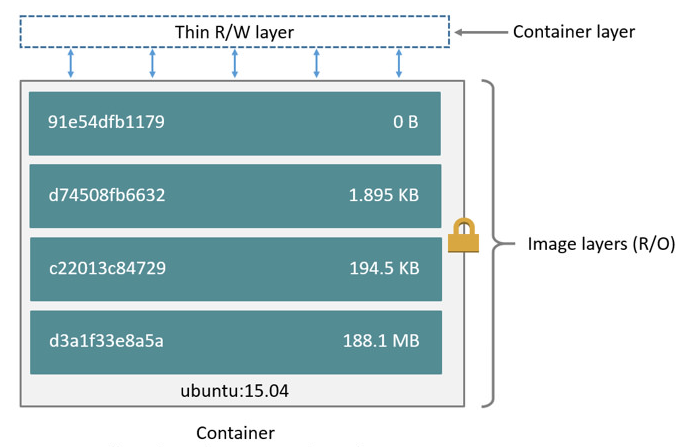
\includegraphics[width=12cm]{ubuntu-container.png}
    \caption{Un Conteneur Docker basé sur l'Image Docker d'Ubuntu.}
    \label{fig:ubuntu-container}
\end{figure}

Dans l’autre côté, un Conteneur Docker est tout simplement l’instance active – avec état - en cours d’exécution d’une Image Docker. C’est similaire au principe des Classes et ses Objets dans la programmation orientée Objets. l’exécution d’un Conteneur Docker signifie la création d’une couche légère et écrivable du système de fichiers – au-dessus des couches enregistrées de l’Image source -, dans laquelle toutes les modification effectuees pendant l’exécution du Conteneur seront sauvegardées, jusqu’à la destruction de ce Conteneur. Cette structure permet à plusieurs Conteneurs de partager la même Image, même plusieurs Images de partager les couches identiques.
\newline

\subsection{GitLab}
Pour les développeurs en particulier, et chaque utilisateur informatique en général, garder la trace des changements effectués sur les fichiers est une fonctionnalité essentielle pour une bonne gestion du code source. La possiblité d’annuler les changements, retourner à une version antérieure d’un fichier, comparer les modifications entre les versions … et plus de fonctionnalités sont les objectifs d’un système de gestion des versions. 
\newline

SVN et Git sont deux exemples des systèmes de contrôle de version open source, avec Git le plus populaire aujourd'hui.

\subsubsection{Git : Gestion des Versions Décentralisé}
Git est un système distribué de contrôle des versions libre et open source, créé en 2005 par Linus Torvalds, fondateur du noyau Linux. Au moment d’écriture de ces lignes, git a arrivé à sa version 2.13. 
\newline

Git offre “toutes” les fonctionnalités fournies par les concurrents du marché, avec l’avantage de la décentralisation, ce qui permet d’utiliser Git de manière similaire en local comme en équipe dans le réseau.
\newline

\textbf{Systèmes de Contrôle des Versions Locaux} \newline
Dans un premier temps, l’approche adopté par les utilisateurs était la copie des fichiers dans un dossier. Cet approche n’était pas efficace car il était souvent sujet à l’erreur si par exemple vous oubliez le dossier sur lequel vous êtes et vous écrasez le – ou les – fichier erroné!


\begin{figure}[H]
    \centering
    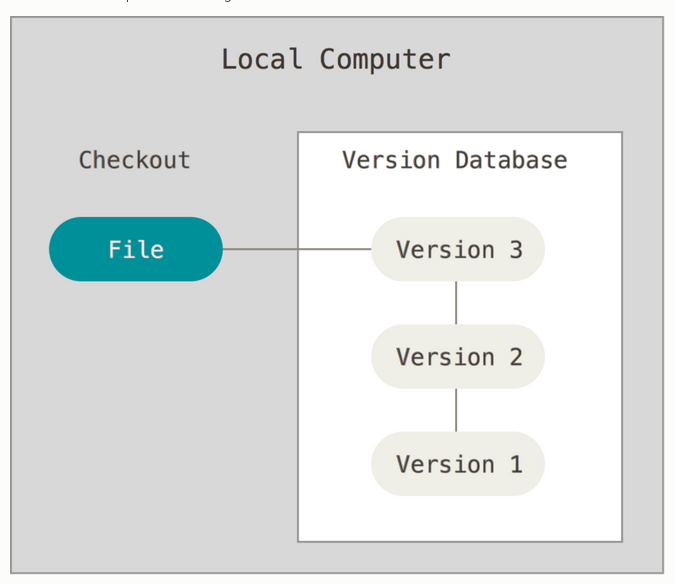
\includegraphics[width=9cm]{local-scm.png}
    \caption{Principe d'un système de contrôle des versions local.}
    \label{fig:local-scm}
\end{figure}

Pour éviter ces accidents, les développeurs ont créé des systèmes de contrôle des versions locaux qui avaient des bases de données qui stockent les changements des fichiers. Le plus populaire de ces systèmes était RCS, qui travaille avec le principe de stocker les différences entre les fichiers – appelées patches - sur le disque sous un format spécial de telle manière qu’il soit capable de restorer le contenu de n’importe quel fichier dans n’importe quel moment en se basant sur les patches.
\newline

\textbf{Systèmes de Contrôle des Versions Centralisés} \newline
Les développeurs avaient besoin de collaborer entre eux mais sur plusieurs systèmes. Pour attaquer ce besoin, les systèmes de contrôle des versions centralisés ont été créés. Ces systèmes comme CVS et SVN ont un seul serveur qui contient toutes les versions des fichiers du code source et un nombre de clients qui copie les fichiers depuis ce serveur central. Cela était le standard pendant plusieurs années.

\begin{figure}[H]
    \centering
    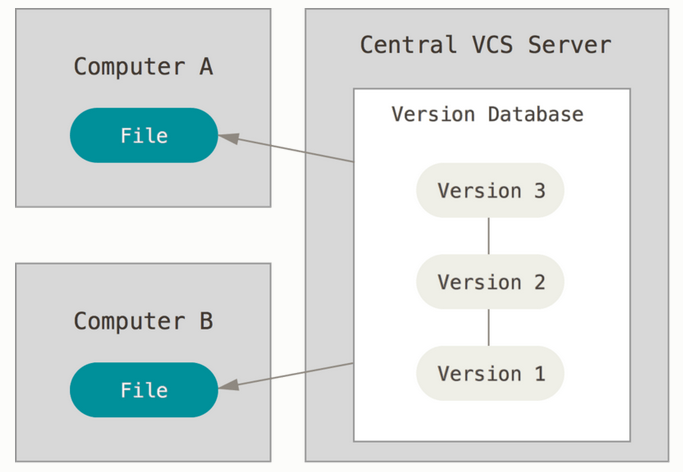
\includegraphics[width=12cm]{central-scm.png}
    \caption{Principe d'un système de contrôle des versions central.}
    \label{fig:central-scm}
\end{figure}

Le point faible majeur de cet approche était le point de défaillance unique; un seul serveur contient tous les fichiers. Si ce serveur tombre en panne, personne ne peut collaborer ou effectuer des échanges avec lui, il y avait même le risque de tout perdre si le support de stockage tombe en panne et pas de backup était effectué. Ces incovénients ont été addressés par les systèmes décentralisés.
\newline

\textbf{Systèmes de Contrôle des Versions Décentralisés} \newline
Au lieu de cloner seulement quelques fichiers depuis le répertoire central, les systèmes de contrôle des versions décentralisés permettent le clonage complet du répertoire, effectuer les changements, et puis pousser le répertoire entier au serveur central à nouveau. Si le serveur central tombe en panne, n’importe quel répertoire chez les utilisateurs peut être copié au nouveau serveur, et continuer la collaboration comme avant. En principe, chaque clone du répertoire central par les utilisateurs est considéré comme un backup complet de ce répertoire!

\begin{figure}[H]
    \centering
    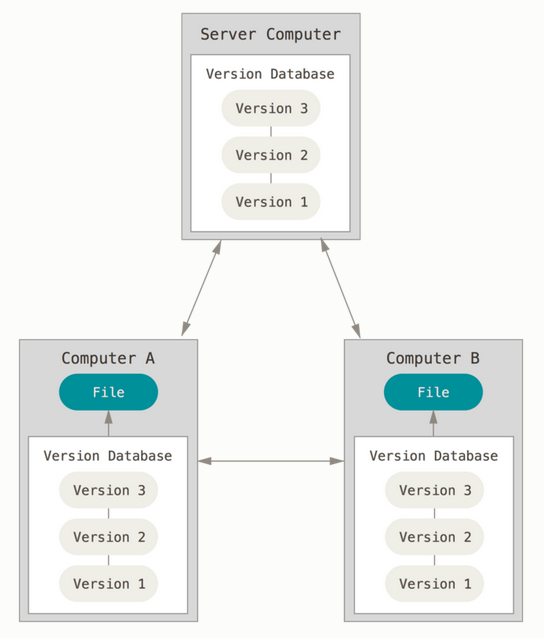
\includegraphics[width=9cm]{distributed-scm.png}
    \caption{Principe d'un système de contrôle des versions distribué.}
    \label{fig:distributed-scm}
\end{figure}

Git et Mercurial sont parmi les systèmes décentralisés les plus populaires, avec Git en top pour sa richesse en termes de fonctionnalité et comme étant un projet libre et open source supporté par une grande communauté et utilisé par les tops entreprises de technologies mondiales.

\subsubsection{C’est quoi GitLab?}
Git est un logiciel basé sur la ligne de commandes, mais pas tout le monde travaille avec elle. Avec les environnements de développement intégrés – IDEs – et les frameworks, les développeurs – et autres – souvent utilisent les interfaces graphiques pour ses tâches quotidiennes, ce qui impose d’avoir des outils graphiques pour Git.
\newline

Alors GitLab est une application web pour la gestion des répertoires Git créée en 2011, similaire à GitHub, développée en langages Ruby et Go. La société GitLab Inc. fournit GitLab en deux produits; une version Communautaire avec une licence open source, et une version Commerciale avec plus de fonctionnalités destinées aux grandes Entreprises.

\begin{figure}[H]
    \centering
    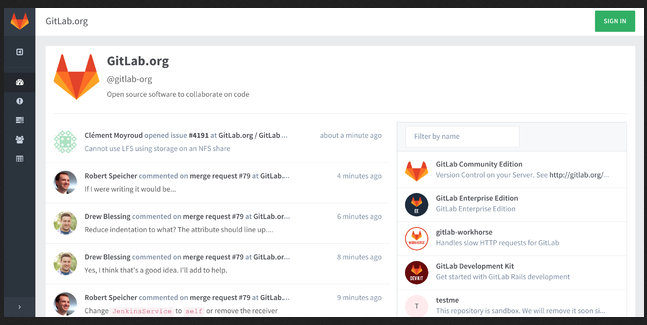
\includegraphics{exemple-gitlab.png}
    \caption{Une interface web sur GitLab.}
    \label{fig:exemple}
\end{figure}

On peut dire que GitLab permet d’avoir notre propre GitHub local. GitLab fournit toutes les fonctionnalités de base de Git, et bien d’autres comme les pipelines l’Intégration/Déploiement Continue , un Wiki intégré, gestion des utilisateurs et groupes d’utilisateurs, nombre de répertoires Git privés et/ou publics illimités, la trace et gestion des problèmes – appelés Issues – et des “A Faire” - appelés Todos - , les notifications , … et autres.
\newline

FY Computing accueille des dizaines de développeurs, webdesigners et sysadmins et veut bénéficier des services comme ceux de GitHub mais hébérgé en local et illimités, alors GitLab était notre choix unique pour cela. Alors on a procédé à hébergé l’application web GitLab à l’aide des Conteneurs Docker.

\subsection{Jenkins}

TO-DO

\subsubsection{CI/CD : Intégration/Déploiement Continue ?}
En principe, le terme Intégration Continue – en anglais Continuous Integration – signifie le processus que, à chaque modification du code source dans le répertoire, le projet en cours de développement doît être compilé, testé et validé de façon automatique en fournissant à la fin un feedback à l’entité responsable de la modification. Le Déploiement Continue – en anglais Continuous Deployment – englobe l’Intégration Continue et lui ajoute l’automatisation de déploiement du projet dans plusieurs environnement d’exécution; test, pré-production et production.
\newline

Cette pratique élimine les problèmes causés par la phase d’intégration des changements effectués sur le code source; par exemple une modification du code qui ne marche pas ou fonctionnalité incomplète. Elle permet aussi d’améliorer la qualité et d’augmenter la rapidité de développement des applications.

\subsubsection{Introduction à Jenkins}
Jenkins est un outil open source d’Intégration Continue développé en Java. C’est un fork de “Hudson” après le dispute du développeur de ce dernier et la société Oracle. Il fonctionne comme étant une application web JavaEE. 
\newline

Jenkins s’intègre nativement avec les projets basé sur le langage de développement Java, mais peut être étendu vers presque n’importe quel autre langage à travers les plugins, ce qui montre sont point fort par rapport à ses concurrents du marché.

\subsection{MySQL Clustering}

Presque chaque application informatique necessite le stockage des donnees, et pour cela elle a besoin d’une – même plusieurs - base de donnees et il y en a plusieurs choix des SGBD – Systèmes de Gestion des Bases de Données. MySQL a été le choix libre et open source le plus populaire depuis longtemps, même avec Percona et MariaDB qui sont des dérivatives de MySQL qui fournissent plus de fonctionnalités.

\subsubsection{Le SGBD MySQL}
MySQL est un SGBD relationnelles. Il est distribué sous une double licence open source GPL et propriétaire. Il fait partie des logiciels de gestion de gestion des bases de données les plus utilisés au monde, autant par le grand public que par des professionnels.

\subsubsection{Les Dérivés Compatibles MySQL}
Après l’acquisition de MySQL par Sun en 2008 puis même cette dernière était acquise par Oracle en 2009, des groupes de développeurs ont quitté MySQL en faveur de la création de leurs propre dérivative  du code source MySQL, ce qui nous donne aujourd’hui MariaDB et Percona. Ces deux dérivatives de MySQL ont été développé pour servir comme remplaçants transparents – c’est à dire 100\% compatible - de MySQL fournie par Oracle.
\newline

Lorsque MariaDB se concentre sur l’innovation et l’ajout des nouvelles fonctionnalitées avancées pour MySQL, Percona essaye d’améliorer au maximum la côté performance du serveur avec l’introduction des solutions de haute performance et de gestion pour les installations compliquées dans le Cloud.
\newline

\subsection{Développement Full Stack avec MEAN.JS}

Lorsqu'on dit "développement Full Stack", on parle du développement de toutes les parties d'un site ou application web, depuis la conception de la base de données et programmation du serveur web dans le Back End jusqu'à l'interface graphique des utilisateurs dans le Front End.
\newline

Le MEAN\cite{gettingMEAN} Stack se compose de 4 technologies principales :
\begin{itemize}
\item \textbf{M}ongoDB - La base de donnees.
\item \textbf{E}xpressJS - Framework de développement Web (Back End).
\item \textbf{A}ngularJS - Framework de développement Web (Front End).
\item \textbf{N}odeJS - Serveur Web.
\newline
\end{itemize}


MongoDB a été créé en 2007 et maintenu par MongoDB Inc., il était anciennement connu sous le nom 10gen.
\newline

ExpressJS est un projet open-source lancé en 2009 par T.J. Holowaychuck et considéré le framework web le plus populaire pour NodeJS.
\newline

AngularJS aussi un projet open-source supporté par Google, il est au marché depuis 2010 et très active en terme de développement et d'innovation.
\newline

NodeJS a été créé en 2009 et se base sur le moteur open-source de JavaScript V8 développé par Google.

\subsubsection{MongoDB}

La persistence des données est une phase indispensable dans le cycle de vie d'une application. Le choix de la base de données dans le MEAN Stack est tombé sur MongoDB, le 'M' dans ``MEAN''. En général, on est habitué au concept des lignes et colonnes dans les bases de données relationnelles, mais MongoDB n'est pas comme ça! MongoDB est un serveur open-source de bases de données orienté document\cite{documentDB} qui est très performant et évolutif.
\newline

Les \texttt{Documents} de MongoDB sont similaires aux objects \texttt{JSON - JavaScript Object Notation}\cite{json}, avec les valeurs des champs peuvent inclure d'autre documents, des tableaux, et des tableaux de documents. Les Documents - aussi connu sous le nom Objets - correspondent à des types de données natives dans plusieurs langages de programmation (comme JavaScript)ce qui reflète un point fort de ce type des bases de données. De plus, les Documents embarqués et les tableaux des Documents réduit le besoin d'effectuer des jointures coûteuses en terme de performance. MongoDB supporte les données semi-structurées, alors il offre de la polymorphisme à travers ses schémas de données dynamiques. Par contre, MongoDB n'est pas une base de données transactionnelle, et ne doit pas être utilisé pour cela\cite{mongoDBAndMySQLCompared}.
\newline

Mongoose est un module de modélisation des objets MongoDB pour NodeJS. Souvent les applications nécessite une modélisation de ces structures de données (et pas la base de données MongoDB elle-même!), donc Mongoose permet la définition d'un schéma de donnée dont on définit quel type de données peut être dans un Document, ou bien quelle donnée doit être dans ce Document ... etc. Plus que la modélisation, Mongoose fournit une toute couche entière de fonctionnalités au dessus de MongoDB, très utiles dans le développement des applications Web (Gestion des connexions à MongoDB, validation des données, lecture et écriture simple de Documents ... etc).\cite{mongooseDocs}

\subsubsection{ExpressJS}

Dans la création des serveurs et applications Web, il y a des tâches commune qui se répètent et on doit les faire à chaque fois. Express est un framework Web pour NodeJS créé pour ce genre de tâches. Sachant que NodeJS est un plateforme et non pas un serveur, Il nous donne la possibilité d'être créative dans la création de notre serveur Web mais un peu difficile pour développer un serveur Web simple. 
\newline

Express adresse cette difficulté en ajoutant une couche d'abstraction au-dessus de NodeJS pour créer un serveur Web qui écoute pour les requêtes et retourne les réponses adéquates. Parmi les avantages d'Express est sont API de routage Web, qui fournit une interface simple pour lier des addresses URL vers un morceau du code source qui peut soit retourner une page HTML, lire depuis une base de données, écrire dans la base de données ... etc. Ceci rend la taĉhe de créer cette même fonctionnalité avec NodeJS beaucoup plus rapide, simple et facile à maintenir.

\subsubsection{AngularJS}

En résumé, AngularJS est un framework JavaScript pour travailler avec les données directement dans le côté Client (i.e. Front End) et basé sur l'architecture \texttt{MVC}\cite{mvcArchitecture}. On peut développer une application Web complète juste avec les autres trois technologies MEAN, mais AngularJS nous permet de déplacer peu des traitements de données dans le côté Serveur vers le côté Client, souvent en laissant le programme du Serveur traite la communication avec la base de données.
\newline

AngularJS se base sur la liaison bidirectionnelle de données (en anglais \texttt{Two-Way Data Binding}) à l'opposée de la liaison unidirectionnelle de données qui est la méthode traditionnelle. Cette dernière est utilisée déjà lorsqu'on développe un projet avec MongoDB, NodeJS et Express seulement; NodeJS récupère les données depuis MongoDB puis Express utilise des modèles (en anglais \texttt{Templates}) pour compiler ces données en HTML délivré par la suite au Client [voir la figure \ref{fig:one-way-data-binding}]. Dans ce genre de liaison, la majorité du travail est effectué dans le côté Serveur. 

\begin{figure}[H]
    \centering
    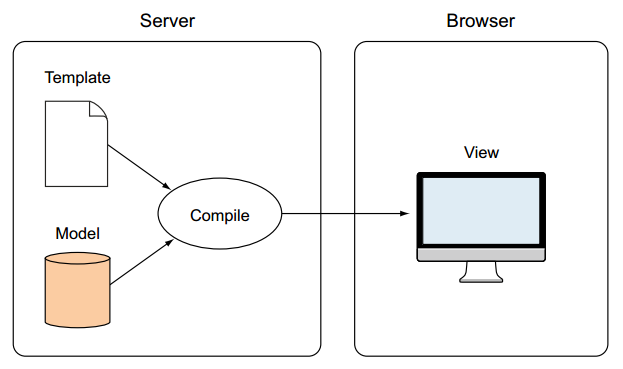
\includegraphics[width=10cm]{one-way-data-binding.png}
    \caption{Liaison unidirectionnelle de données dans le côté Serveur.}
    \label{fig:one-way-data-binding}
\end{figure}

Par contre, la liaison bidirectionnelle des données est différente. \texttt{Template} et les données sont envoyées séparémment au client Web. Le client Web est maintenant responsable de compiler le \texttt{Template} en une vue HTML et les données en \texttt{Model}. La différence majeure est que la Vue est ``vivante'', cest-à-dire si le \texttt{Model} change, la \texttt{View} reflète ce changement instantanémment, et vice-versa [voir la figure \ref{fig:two-way-data-binding}].

\begin{figure}[H]
    \centering
    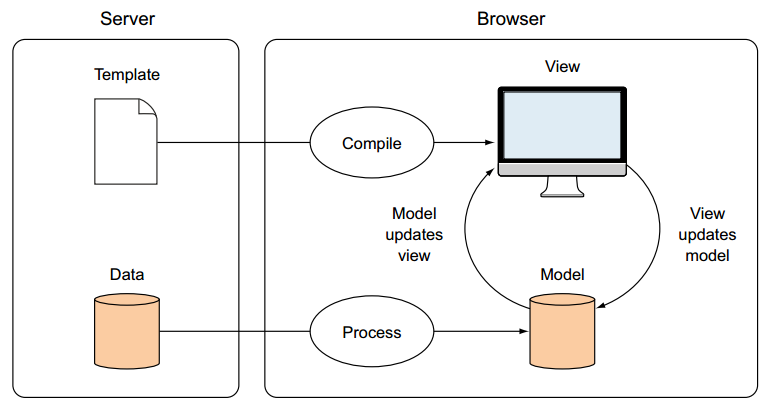
\includegraphics[width=11cm]{two-way-data-binding.png}
    \caption{Liaison bidirectionnelle de données avec AngularJS dans le côté Client.}
    \label{fig:two-way-data-binding}
\end{figure}

\subsubsection{NodeJS}

NodeJS est la fondation du MEAN Stack. NodeJS est un environnement JavaScript de côté serveur qui est évènnementiel avec des requêtes d'entrée et de sortie non-bloquantes et basé sur le moteur JavaScript V8 de Google. En résumé, NodeJS nous permet de créer notre serveur Web avec nos applications web en top. Il n'est pas un langage ni un serveur Web lui-même, mais contient une bibliothèque de serveur HTTP, ce qui veut dire qu'on n'aura pas besoin d'avoir un serveur Web externe (Apache, Internet Information Services ``IIS'' ...) pour exécuter nos projets Web. Malgré que ceci nous donne un contrôle étendu sur la façon comment notre serveur Web fonctionne, mais il complique la tâche de sa création et son lancement rapide.
\newline

Un serveur Web créé par NodeJS est \texttt{``single-threaded''}, cest-à-dire tous les clients seront servi par un seul thread, le même thread. Cet approche est différent aux autres serveurs Web qui sont considérés \texttt{``multithreaded''} (comme Apache) qui affectent un thread pour chaque connexion d'un client. De plus, les évènnement d'entrée et de sortie pour NodeJS sont non-bloquants\cite{blockingVSnonBlocking}, ce qui permet à l'application web de ne pas se bloquer en attente des résponses aux requettes vers les ressources sur le système, et cela permet à NodeJS d'être beaucoup plus rapide\cite{nodeJSvsPHP}.
\newline

NPM est un gestionneur des modules installé avec NodeJS. Il nous donne la possibilité de télécharger des modules NodeJS pour étendre les fonctionnalités de nos applications. Au moment de la rédaction, NPM héberge presque demi-million de modules gratuitement ce qui montre combien de fonctionnalités prêtes à utiliser qui peuvent être ajoutées à nos applications NodeJS.

\newpage

\chapter{Réalisation du Projet}

\newpage

\chapter*{Conclusion et Perspectives}

\newpage

\renewcommand{\appendixtocname}{Annexes}

\begin{appendices}

\chapter{Installation et Configuration Docker sur Ubuntu Server}
Jusqu'à maintenant, Docker ne peut s'installer que sur les systèmes 64 bits, c'est à dire que votre système Linux ou autres (Windows, macOS) doit être 64 bits. Pour les utilisateurs de Windows et macOS, ils peuvent installer Docker sur une VM de Linux ou sur leurs propre machine avec Docker for Windows et Docker for macOS. Dans cet annexe, je vais me focaliser dans les prochaines paragraphes sur les étapes d'installation de Docker Engine (CE) sur Ubuntu Server version 16.04 LTS.

\section{Installation Manuelle}

Cette partie montre les étapes détaillées d'installation de \texttt{Docker Engine} sur le système \texttt{Ubuntu Server}. La partie suivante donne la possibilité d'automatiser ces étapes pour une installation rapide et transparente.

\subsection{Préparation des Dépendances}
Comme la majorité des applications, Docker se base sur plusieurs dépendances applicatives qui doivent être installées au préalable pour son bon fonctionnement. D'après sa documentation\cite{dockerDocs} officielle, Docker a besoin de l'installation des dépendances suivantes :
\usemintedstyle{vim}
\begin{minted}{shell}
sudo apt-get update && apt-get install -y --no-install-recommends \
     apt-transport-https \
     ca-certificates \    
     curl \     
     gnupg2 \     
     software-properties-common
\end{minted}
L'option ``--no-install-recommends'' empêche le gestionnaire des paquetages APT d'installer d'autres programmes recommandés.
\newline

Ensuite, avant d'installer le répertoire de Docker sur APT, ce dernier aura besoin de vérifier sa clé d'authentification GPG, qu'on doit l'apporter à APT à l'aide de la commande suivante :
\begin{minted}{shell}
curl -fsSL https://download.docker.com/linux/ubuntu/gpg | sudo apt-key add -
\end{minted}

Et maintenant on est prêt à ajouter le répertoire APT de Docker pour Ubuntu :
\begin{minted}{shell}
sudo add-apt-repository \
  "deb [arch=amd64] https://download.docker.com/linux/ubuntu $(lsb_release -cs) stable"
\end{minted}
``\$(lsb\_release -cs)'' est une commande Shell qui retourne le codename de la version installé de votre distribution Linux!
\subsection{Installation de Docker Engine - CE (Community Edition)}

Après avoir préparé les dépendances systèmes, Docker peut être installé maintenant à l'aide de la commande ci-dessous qui permet l'installation de la dernière version stable de Docker Engine, ce qui est souvent recommandé.
\begin{minted}{shell}
sudo apt-get update && sudo apt-get install -y docker-ce
\end{minted}

Afin de tester que l'installation s'est terminé avec succès, la commande suivante permet le téléchargement d'une Image Docker de test et va l'exécuter dans un Conteneur sur votre machine. 
\begin{minted}{shell}
sudo docker run hello-world
\end{minted}

Normalement, si aucune erreur ne s'est produit pendant le processus d'installation, la commande ci-dessus doit afficher le message suivant - et autres - indiquant le bon fonctionnement de Docker Engine :
\newline
{\scriptsize
  \emph{
    \textbf{\\
    Hello from Docker!\\
    This message shows that your installation appears to be working correctly.
    }
  }
}

\subsection{Configuration Post-Installation de Docker Engine}

Lors de l'installation, Docker crée un groupe d'utilisateurs "docker" dont, au départ, seulement l'administrateur du système fait partie. La commande suivante permet à un compte utilisateur courant de joindre ce groupe pour éviter d'exécuter les commandes Docker à chaque fois en mode root avec "sudo" :

\begin{minted}{shell}
sudo usermod -aG docker $USER
\end{minted}

Pour que pour cette commande prenne effet, il faut se déconnecter et puis reconnecter à votre session de connexion Linux. Si vous essayez Docker sur une machine virtuelle Linux, il se peut parfois qu'elle requière un redémarrage complet!.
\newline

Si on veut que le démon Docker démarre avec le système, on doit en achever en executant la commande suivante qui permet le lancement automatique du service Docker au moment du démarrage du systeme Linux :

\begin{minted}{shell}
sudo systemctl docker enable
\end{minted}


Et voilà! On est le bienvenue à un tout nouveau monde des Conteneurs avec Docker.

\newpage

\section{Installation Automatisée}

Pour une installation transparente et rapide, j'ai créé un script Bash qui automatise la procédure d'installation de Docker Engine sur Debian/Ubuntu. Il suffit d'exécuter les quatres commandes suivantes pour télécharger le script d'installation puis installer la derniere version stable de Docker Engine sur votre machine :

\begin{minted}{shell}
# Téléchargement du script Shell
sudo wget \
  https://raw.githubusercontent.com/elouizbadr/cluster/master/install_docker_debian.sh

# La commande ci-dessous est à exécuter par les utilisateurs du système Ubuntu
# et à ignorer par les utilisateurs du système Debian.
export OSNAME=ubuntu 

# Lancement du script Shell
sudo chmod +x ./install_docker_debian.sh && sudo ./install_docker_debian.sh
\end{minted}

\chapter{Préparation d'un Environnement MEAN Stack sur Ubuntu Server}

\newpage

\section{Installation et Configuration de MongoDB}
Malgré qu'Ubuntu fournit ces propres paquetages d'installation MongoDB, il est souvent recommandé d'installer MongoDB depuis ses paquetages officiels, qui sont en général à jour. MongoDB fournit seulement les paquetges d'installation pour la version 64 bits d'Ubuntu LTS, qui peuvent marcher bien avec les autres version non-LTS mais ils ne sont pas supportés.
\newline

MongoDB fournit ses paquetages officiels suivant dans son propre répertoire :
\begin{itemize}
  \item{\textbf{mongodb-org} : Un meta-paquetage qui installe automatiquement les quatres paquetages ci-dessous.} 
  \item{\textbf{mongodb-org-server} : Contient le démon \textbf{mongod} et ses fichiers de configuration et de démarrage.} 
  \item{\textbf{mongodb-org-mongos} : Contient le démon \textbf{mongos}.} 
  \item{\textbf{mongodb-org-shell} : Contient le shell \textbf{mongo}.} 
  \item{\textbf{mongodb-org-tools} : Contient d'autres outils d'administration MongoDB.} 
  \newline
\end{itemize}


Les paquetages ci-dessus entrent en conflit avec les paquetages \textbf{mongodb, mongodb-server} et \textbf{mongodb-clients} fournit par Ubuntu. 
\newline

Le fichier de configuration par défaut de MongoDB \textbf{/etc/mongod.conf} contient le paramètre \textbf{bind\_ip 127.0.0.1} par défaut, ce qu'oblige le démon \texttt{mongod} à servir seulement les requêtes qui proviennent de la machine locale. Pour servir autres clients dans le réseau si vous voulez, il faut changez l'adreese configurée vers une des interfaces réseau configurées de la machine, ou \textbf{*} pour utiliser toutes les interfaces réseau disponibles.
\newline

Alors, afin d'installer MongoDB sur Ubuntu 16.04 LTS, il faut suivre les étapes suivantes :
\begin{enumerate}
  \item{Importer la Clé Publique GPG Utilisée par APT}
  \begin{minted}{shell}
  sudo apt-key adv \
    --keyserver hkp://keyserver.ubuntu.com:80 
    --recv 0C49F3730359A14518585931BC711F9BA15703C6
  \end{minted}

  \item{Créer un fichier \texttt{list} pour APT}
  \begin{minted}{shell}
  echo "deb [ arch=amd64,arm64 ] \ 
    http://repo.mongodb.org/apt/ubuntu xenial/mongodb-org/3.4 multiverse" | \ 
    sudo tee /etc/apt/sources.list.d/mongodb-org-3.4.list
  \end{minted}

  \item{Mettre à jour la base de données APT}
  \begin{minted}{shell}
  sudo apt-get update
  \end{minted}

  \item{Installer les paquetages de MongoDB}
  \begin{minted}{shell}
  sudo apt-get install -y mongodb-org
  \end{minted}

  \item{Lancer le Serveur MongoDB}
  \begin{minted}{shell}
  sudo service mongod start
  \end{minted}
\end{enumerate}

\newpage

\section{Installation de NodeJS}

NodeJS pour Debian et Ubuntu est fournit par le répertoire \texttt{NodeSource}. NodeJS peut être installé sur Ubuntu 12.04 LTS (les deux architectures) ou ultérieure. La politique de distribution des versions de NodeJS est similaire à Ubuntu, avec une version LTS supportée pour une longue durée, et autres versions de développement de temps en temps. A la date d'écriture de ce document, la version LTS de NodeJS était 6.X, donc c'est la version qu'on va installer par la suite.
\newline

\texttt{NodeSource} fournit un script Shell qui facilite la tâche d'installation, donc on l'importe puis l'exécute à l'aide de la comande suivante :
  \begin{minted}{shell}
  curl -sL https://deb.nodesource.com/setup_6.x | sudo -E bash -
  \end{minted}

Enfin, il suffit d'installer le paquetage \texttt{nodejs} avec APT :
  \begin{minted}{shell}
  sudo apt-get install -y nodejs
  \end{minted}

Pour vérifier le bon fonctionnement de NodeJS, vérifiez sa version avec :
  \begin{minted}{shell}
  node --version
  \end{minted}
\newpage

\section{Installation d'ExpressJS et d'AngularJS}

\subsection{Installation d'ExpressJS}
Supposons qu'on a déjà installé NodeJS, on crée le dossier de notre projet d'application :
  \begin{minted}{shell}
  mkdir mon-projet-mean
  cd mon-projet-mean
  \end{minted}

Ensuite, à l'aide du \texttt{npm}, le gestionnaire des modules NodeJS, on crée le fichier \texttt{\emph{package.json}} qui va contenir les métadonnées sur notre projet et ses dépendances :
  \begin{minted}{shell}
  npm init
  \end{minted}
La commande ci-dessus va poser plusieurs questions à propos du projet, pour simplifier la vie, on ira avec les réponses fournies par défaut.

Pour installer le module ExpressJS, il suffit de lance la commande suivante :
  \begin{minted}{shell}
  npm install express --save
  \end{minted}
L'option \texttt{``---save''} permet l'ajout de ce module à la liste des dépendances exprimées dans \texttt{\emph{package.json}}. Vous pouvez installer ExpressJS temporairement à l'aide de l'option \texttt{``---no-save''} ou globalement - disponible partout et pas seulement à ce projet - avec \texttt{``---global''}.

\subsection{Installation d'AngularJS et Twitter Bootstrap}
Les applications et sites Web sont développé à l'aide de plusieurs paquetages; frameworks, bibliothèques, outils ... etc. Garder la trace de tous ces paquetages et les gérer est une tâche difficile et prend beaucoup du temps, c'est pour cela qu'on a besoin d'un gestionnaire qui fait tout ça!

\subsubsection{Bower: Gestionnaire des Paquetages pour le Web}
Bower est un module NodeJS qui gère les dépendances pour le côté client des applications Web. Sa mission principale est d'installer les bonnes versions des paquetages et leurs dépendances dont on a besoin. Avant d'installer Bower, il faut avoir \texttt{NodeJS} et \texttt{git} déjà installés.
\newline

Bower est un outil basé sur la ligne des commandes qu'on peut installer avec :
  \begin{minted}{shell}
  npm install --global bower
  \end{minted}

Pour installer un paquetage, la commande \texttt{bower install} est utilisé. Cette dernière prends comme argument le nom du package, un raccourci GitHub, un répertoire Git, ou un lien URL direct. L'ajout de l'option \texttt{\emph{``---save''}} permet la sauvegarde de ce paquetage dans \texttt{\emph{bower.json}}.
\newline

Une autre méthode d'installation des paquetages Web avec Bower est à travers l'utilisation du fichier \texttt{\emph{bower.json}} qui contient la définition de ces paquetages. Si cette méthode est utilisée, lancez \texttt{bower install} dans le même dossier de \texttt{\emph{bower.json}}. 
\newline

Par défaut, Bower install les paquetages dans le dossier \texttt{\emph{bower\_components}}.

\subsubsection{AngularJS et Twitter Bootstrap avec Bower}
Pour notre projet d'application dans ce rapport, on a utilisé la version 1.x d'AngularJS. Au moment d'écriture de ce rapport, les créateurs d'AngularJS ont arrivée à la version 4.x sour le nom ``Angular'' (sans ``JS''). la version 1.x est complètement incompatible avec les versions 2.x ou ultérieures. Pour installer la dernière version d'AngularJS 1.x, son paquetage est nommé \texttt{\emph{angularjs}}.Les versions 2.x ou ultérieures d'Angular ne sont pas disponibles sur Bower.
\newline

Alors, l'installation d'AngularJS est simple avec Bower :
  \begin{minted}{shell}
  bower install --save angularjs
  \end{minted}

Bootstrap est un framework HTML, CSS et JS qui contient des composants Web prêts à utiliser dans le projet. Bootstrap facilite la phase d'estèthique et d'animation des applications et sites Web.
\newline

Pour installer Twitter Bootstrap avec Bower, il suffit d'exécuter :
  \begin{minted}{shell}
  bower install --save bootstrap
  \end{minted}

\end{appendices}

\bibliographystyle{ieeetr}

\bibliography{Bibl}

\newpage

\end{document}
